% Fokus auf den Treibhauseffekt, d.h. vorherige Abbildung reduziert um ein paar Energieflüsse  (mitte)
% zB Sonneneinstrahlung- Atmosphärische Reflexion = 235 W/m2
% Die Abbildung zeigt zum einen die Temperatur auf der Erde ohne die Strahlungsbilanz der Erde(links) außerdem nochmal den atmosphärischen Aufbau (rechts)
% In der Mitte ist die Auswirkung der Treibhausgase zu sehen

\begin{frame}
  \frametitle{Treibhauseffekt}
  \only<1|handout:0>{
  \begin{figure}
  	\centering
  	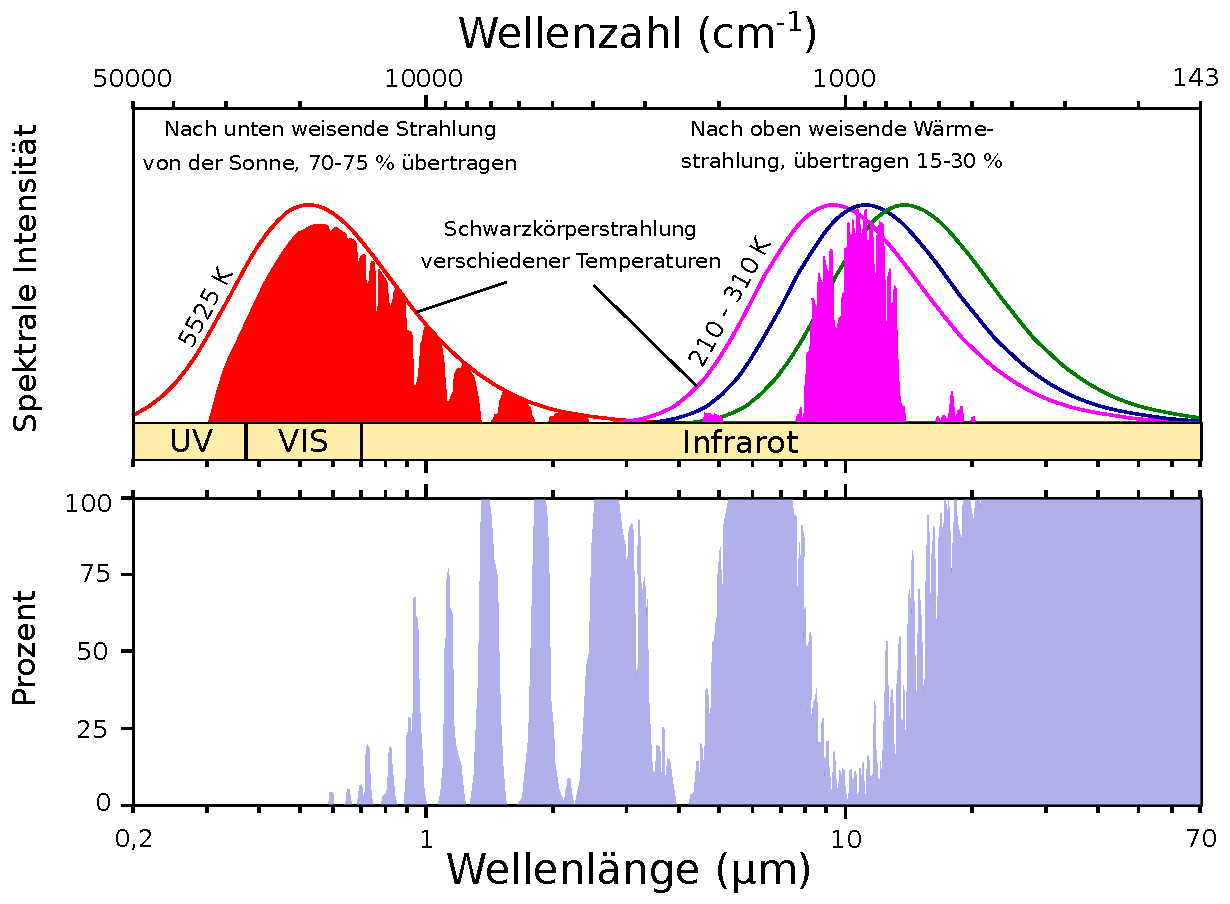
\includegraphics[width=0.7\linewidth]{bilder/Atmospheric_Transmission-H2O.pdf}
    \caption{Absorption und Streuung von Wasser in der Atmosphäre, Quelle: Robert A. Rohde, Global Warming Art project}
  \end{figure}
    }
    \only<2|handout:0>{
    \begin{figure}
    	\centering
    	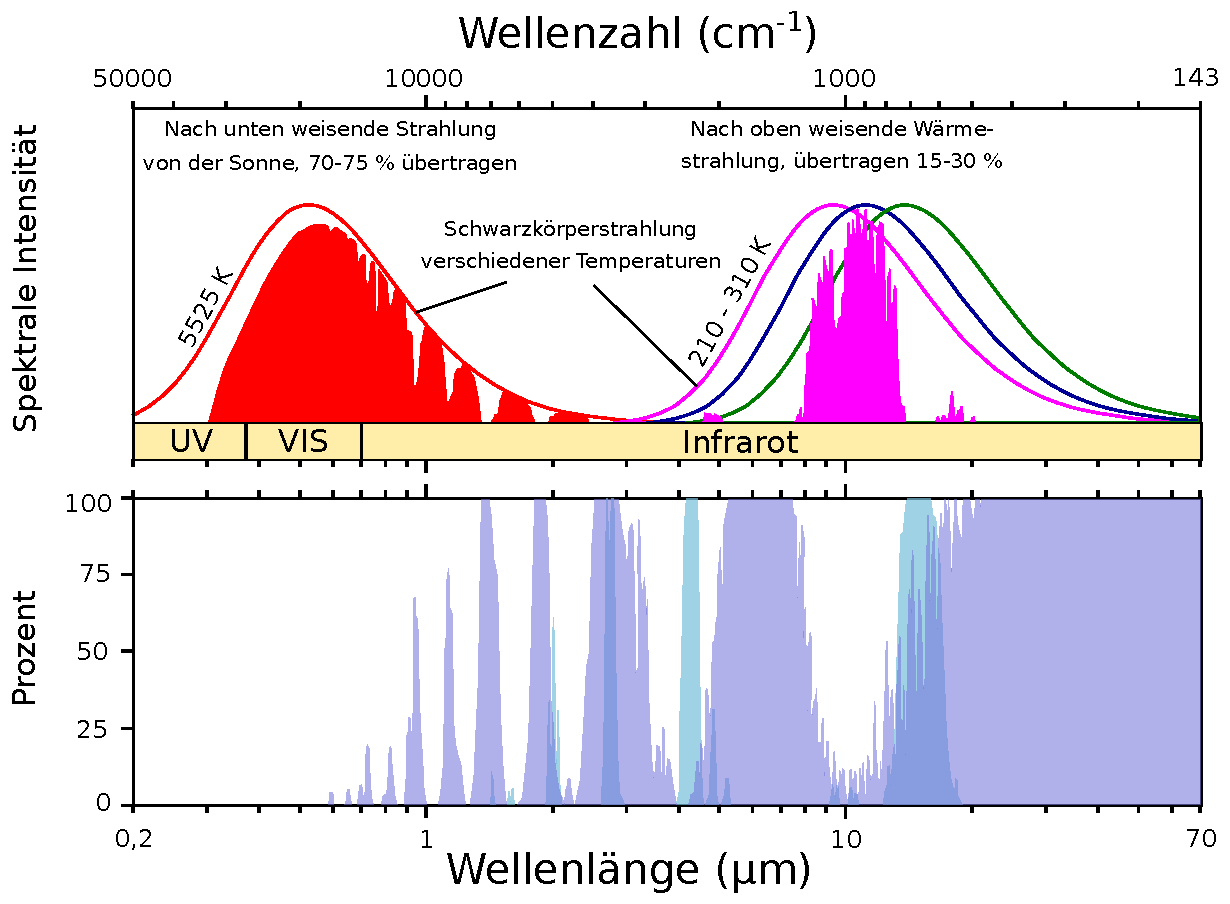
\includegraphics[width=0.7\linewidth]{bilder/Atmospheric_Transmission-H2O-CO2.pdf}
      \caption{Absorption und Streuung von Wasser und CO$_2$ in der Atmosphäre, Quelle: Robert A. Rohde, Global Warming Art project}
    \end{figure}
    }
    \only<3|handout:0>{
    \begin{figure}
    	\centering
    	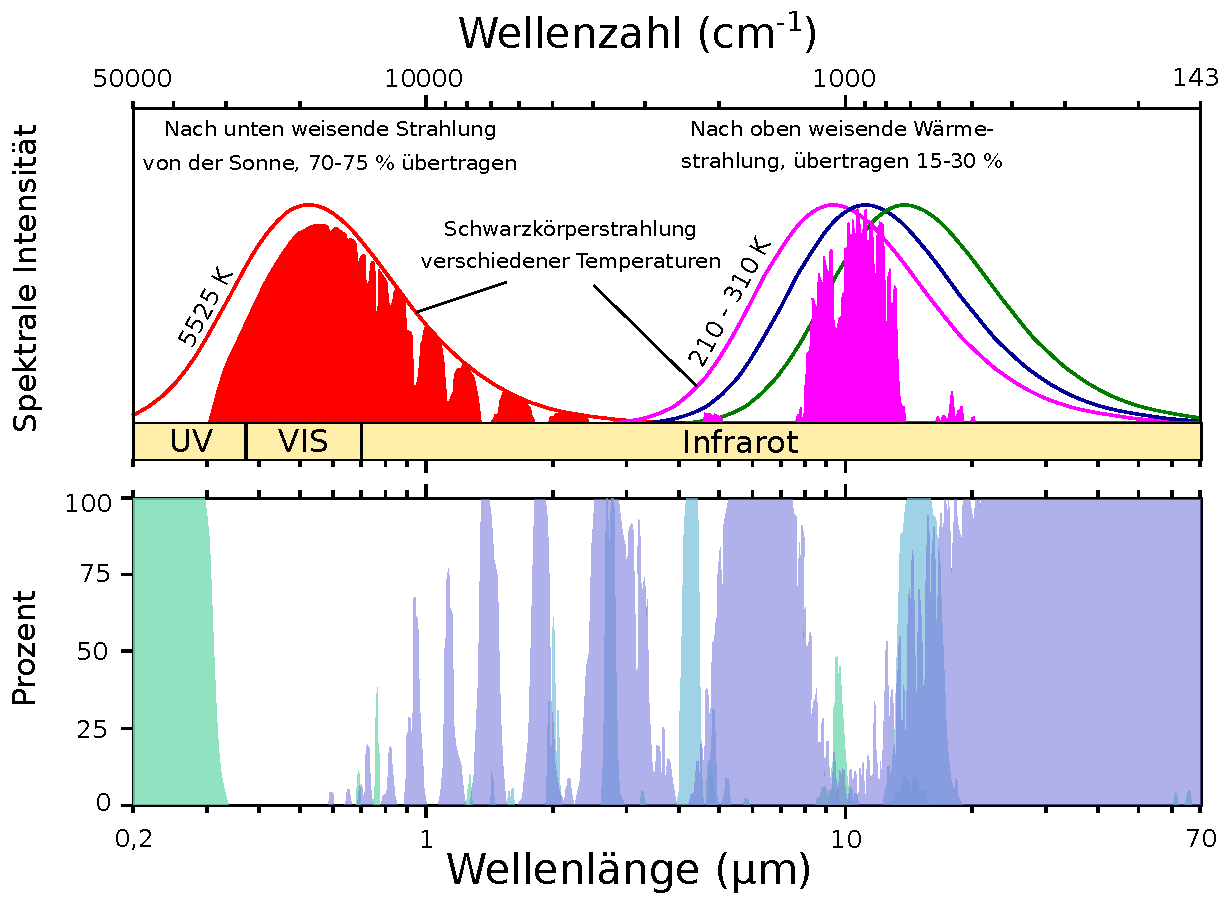
\includegraphics[width=0.7\linewidth]{bilder/Atmospheric_Transmission-H2O-CO2-O2O3.pdf}
    \caption{Absorption und Streuung von Wasser, CO$_2$, sowie Sauerstoff und Ozon in der Atmosphäre, Quelle: Robert A. Rohde, Global Warming Art project}
  \end{figure}
    }
    \only<4|handout:0>{
    \begin{figure}
    	\centering
    	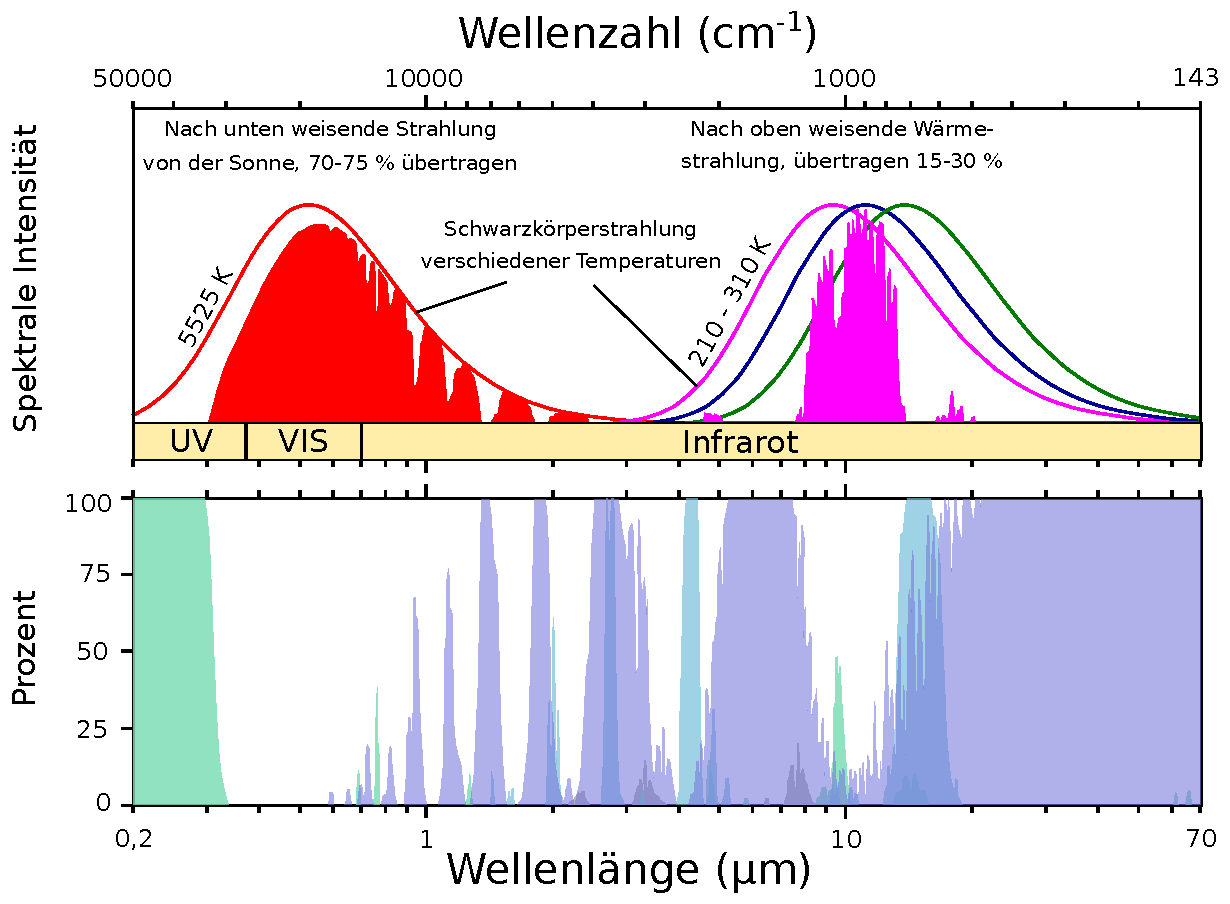
\includegraphics[width=0.7\linewidth]{bilder/Atmospheric_Transmission-H2O-CO2-O2O3-CH4.pdf}
    \caption{Absorption und Streuung von Wasser, CO$_2$, Sauerstoff, Ozon und Methan in der Atmosphäre, Quelle: Robert A. Rohde, Global Warming Art project}
  \end{figure}
    }
    \only<5>{
    \begin{figure}
    	\centering
    	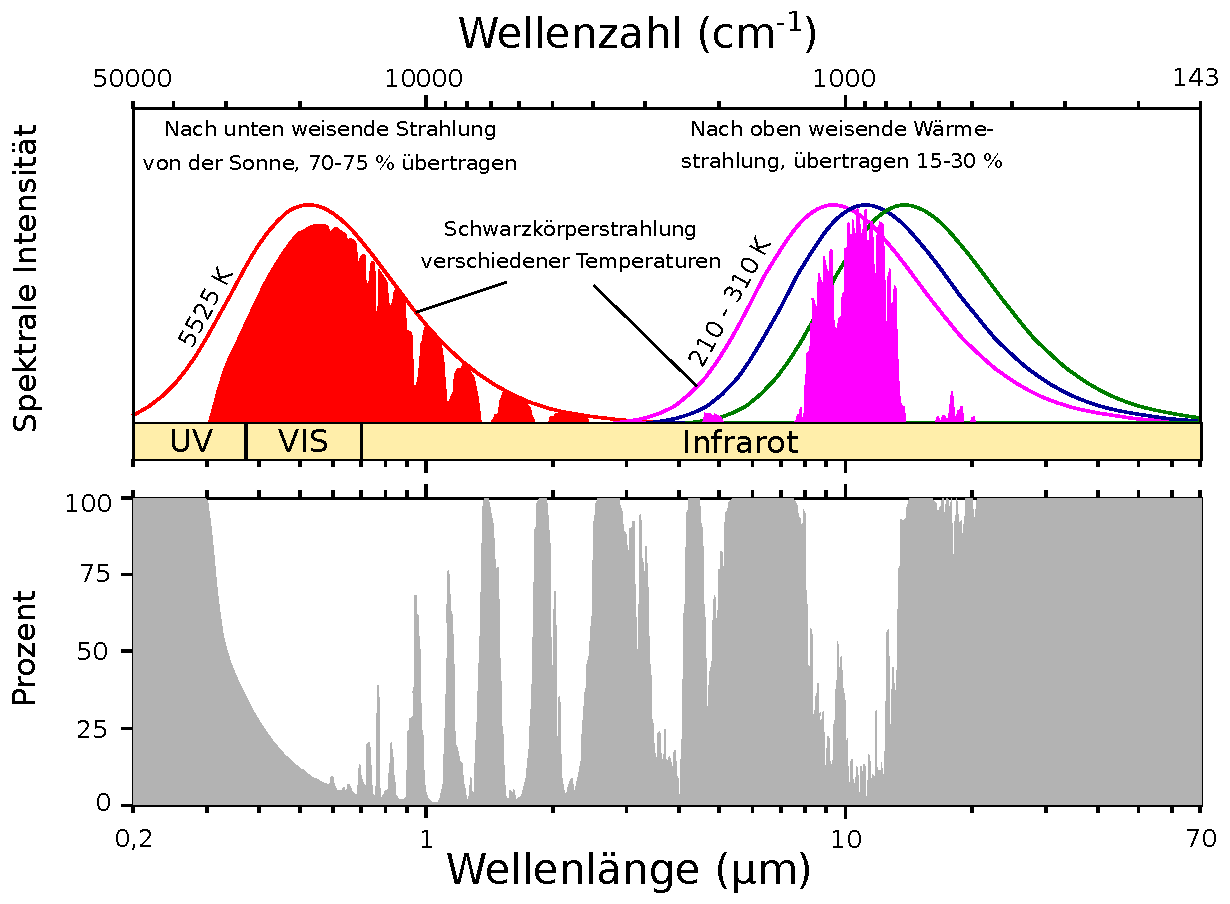
\includegraphics[width=0.7\linewidth]{bilder/Atmospheric_Transmission-all.pdf}
    \caption{Gesamtabsorption und -streuung der Atmosphäre, Quelle: Robert A. Rohde, Global Warming Art project}
  \end{figure}
    }

  \note{
  \begin{itemize}
    \item[] Thermische Ausstrahlung der Erde etwa \SI{240}{W\per m\squared}
    \item[$\rightarrow$] entspricht einer Strahlungstemperatur von etwa \SI{-20}{°C} (Plancksches Strahlungsgesetz, Wärmestrahlung eines schwarzen Körpers)
    \item[] tatsächlich beobachtete Temperatur aber \SI{35}{°C} höher, Wie ist das möglich?
		\item  {\color{red}{Wasserdampf H$_2$O}} -  großer Teil des natürlicher Treibhauseffekt (\SI{60}{\%})
		\item  {\color{red}{Kohlenstoffdioxid CO$_2$}} - entsteht u.A. bei der Nutzung fossiler Brennstoffe (Öl, Kohle, Gas)
    \item[$\rightarrow$] Anstieg auf den Menschen zurückzuführen
    \item  {\color{red}{Ozon O$_3$}} - entsteht bei Reaktion von Auto-Abgasen in der Luft im Sonnenlicht
		\item  {\color{red}{Methan CH$_4$}} - entsteht u.a. bei der Zersetzung von organischem Material
		\item[$\rightarrow$] $>$ 60\,\% der globalen Methan-Emissionen sind auf menschliche Aktivitäten zurückzuführen %ClimateChange Kurs der Uni Helsinki Chapter 1.3.3
		\item  {\color{red}{Distickstoffmonoxid N$_2$O (Lachgas)}} - entsteht beim Abbau von Düngemitteln in der Erde
		\item {\color{red}{fluorierte Treibhausgase (F-Gase)}}
		\item[$\rightarrow$] kommen nicht natürlich vor, sehr treibhauswirksam, verweilen z.T. sehr lange in der Atmosphäre, bis zu 10.000 Jahre, aber kommen nur in sehr geringer Konzentration vor
    \item[] F-Gase: voll halogenierte Fluorkohlenwasserstoffe (FKW, englisch: PFC), teilhalogenierte Fluorkohlenwasserstoffe (HFKW, englisch: HFC), Schwefelhexafluorid (SF6) und Stickstofftrifluorid (NF3).
		\item[] F-Gase kommen in der Natur nicht vor; aber befinden sich u.a. in Gefriertruhen, Klimaanlagen, Feuerlöschern und Dämmstoffen.
	\end{itemize}
  }
\end{frame}

\begin{frame}
	\frametitle{Treibhausgase}
	\begin{figure}
		\centering
    \begin{columns}
      \column{0.7\linewidth}
        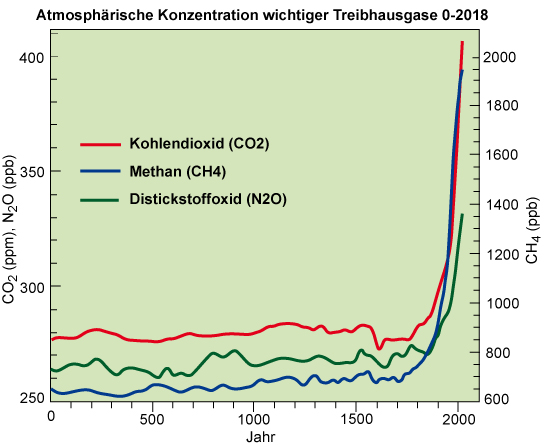
\includegraphics[width=\linewidth]{bilder/Treibhausgase0-aktuell_bildungsserver_hh.jpg}
      \column{0.3\linewidth}
        \caption{Treibhausgaskonzentration in der Atmosphäre, Quelle: Bildungsserver Hamburg}
    \end{columns}
		%Abbildung wie in S.Ranmstorf S.33 -> http://www.pik-potsdam.de/~stefan/Publications/Book_chapters/Der_Klimawandel_Kapitel2.pdf oder direkt im IPCC 2013: https://www.ipcc.ch/report/ar5/wg1/observations-atmosphere-and-surface/ Fig 2.1-2.3
	\end{figure}
\note{
  \begin{itemize}
    \item[] All diesen Stoffen gemeinsam ist ein sehr starker Anstieg der Konzentration seit Beginn der Industrialisierung
    \item[] Der Anstieg ist in absoluten und relativen Zahlen sehr signifikant
    \item[] In dieser Geschwindigkeit ist der Anstieg in der Erdgeschichte beispiellos
    \item[] Die Erhöhung kann im wesentlichen auf menschliche Aktivitäten zurückgeführt werden und setzt sich in Zukunft sehr wahrscheinlich weiter fort
  \end{itemize}
  }
\end{frame}



\begin{frame}
	\frametitle{Treibhausgase - Klimawirksamkeit}
		\begin{figure}
			\begin{columns}
				\column{0.6\linewidth}
				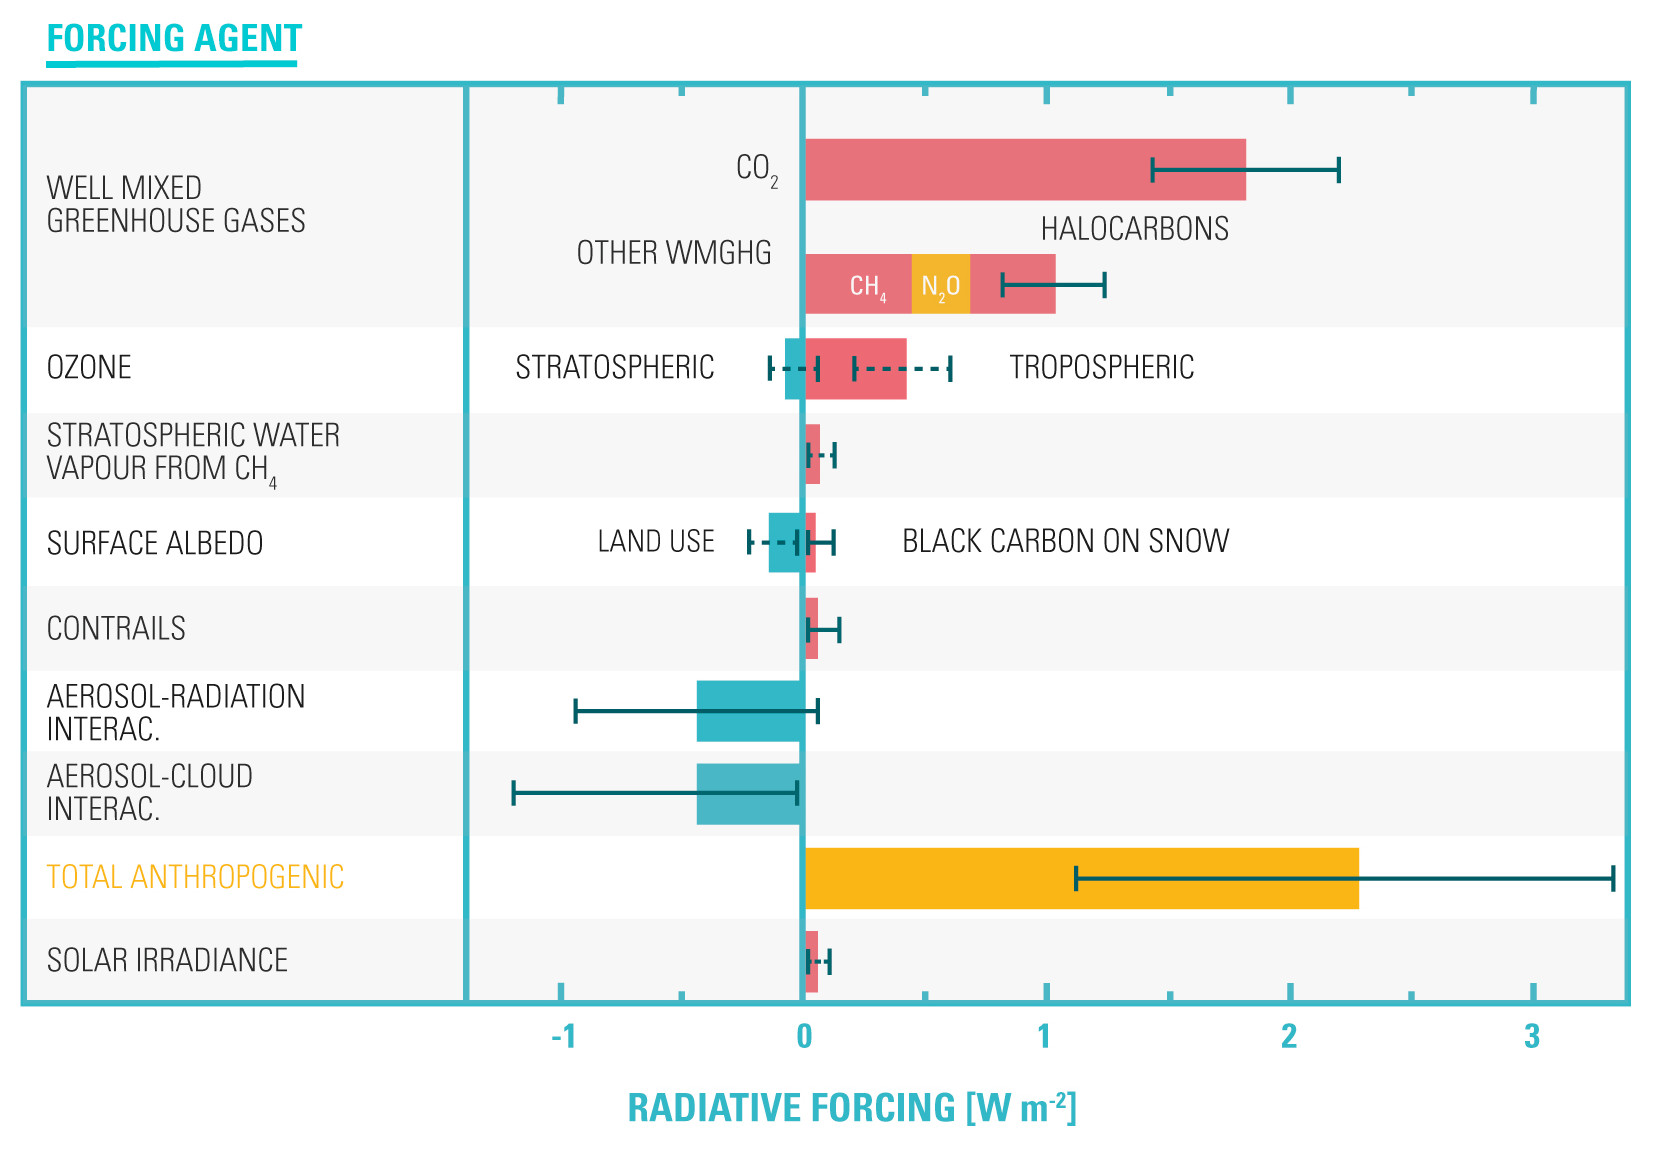
\includegraphics[width=0.9\linewidth]{bilder/radiative_forcing_CCnow_mooc.jpg}
				\column{0.3\linewidth}
				\caption{Strahlungsantrieb der Treibhausgase zwischen 1750 und 2011, Quelle: Climate.now MOOC, abgewandelt von IPCC 2014 Kapitel 8}
			\end{columns}
		\end{figure}
\begin{itemize}
	\item Die Änderungen des Strahlungsantriebs sind durch den Menschen verursacht (ersichtlich durch den betrachteten Zeitraum und das Emissionsquellen bekannt sind)
	\item CO$_2$, CH$_4$ und N$_2$O zählen zu den langlebigen Treibhausgasen und sind über den Globus verteilt.
	\item Der Grad des wissenschaftlichen Verständnisses über diese ist hoch!
\end{itemize}
\note{
  \begin{itemize}
    \item[] Neben den Treibhausgasen beeinflussen weitere Faktoren den globalen Strahlungsantrieb (Energiebilanz der Erde)
    \item[] Diese sind im allgemeinen gekoppelt, z.B. beim Abschmelzen von Eismassen auf Grund von höherer Temperatur
   	\item[] Manche Faktoren wirken dämpfend auf den Strahlungsantrieb, etwa eine erhöhte Aerosolkonzentration
   	\item[] Der Einfluss der Veränderung der Sonnenaktivität (gerne genannten Argument gegen menschgemachten Klimawandel) ist hingehen vergleichsweise klein
   	\item[] Insgesamt gibt es aber (trotz einiger bestehender Unsicherheiten) eine eindeutige Erhöhung des Stralungsantriebs durch menschliche Aktivitäten
    \item[] Contrails = Condensation Trails
    \item[] O$_3$ ist kontinental bis global verbereitet und das Verständnis ist Mittel
  	\item[] CH$_4$ ist global verbreitet jedoch ist das Verständnis über den Strahlungsantrieb gering.
  	\item[] Das Verständnis sinkt nach Einträgen und daher besonders für die verringernden RF-Faktoren wie Albedo ungewiss. Die Verringerung könnte auch deutlich niedriger liegen, was bedeutet, dass der von den Menschen verursachte Strahlungsantireb sogar noch stärker ist. - Da durch die Erderwärmung und Rußablagerungen auf dem Eis der Albedo-Effekt geschmälert wird, ist das sogar wahrscheinlich.
  	% Ergänzungen aus der Abbildung: https://wiki.bildungsserver.de/klimawandel/index.php/Strahlungsantrieb
  \end{itemize}
  }
\end{frame}


\begin{frame}
	\frametitle{CO$_2$-Äquivalent}

	\begin{block}{Strahlungsantrieb / Radiative Forcing / RF}
		Strahlungsenergie pro Quadratmeter, die durch die Tropopause hindurch kommt \\
		Einheit: \SI{}{\watt\per\square\meter}
	\end{block}

	\begin{block}{CO$_2$-Äquivalent}
		Integral des Strahlungsantriebs eines Treibhausgases über einen bestimmten Zeitraum (meist 100 Jahre) im Verhältnis zu dem von CO$_2$

%		Beitrag eines Treibhausgases zum Treibhauseffekt über 100 Jahre gemessen am Beitrag des $CO_2$
	\end{block}


	\color{gray}\rule{\linewidth}{1pt}

	\color{black}

	2018 lag der Wert an CO$_2$-Äquivalenten in der Atmosphäre bei 496\,ppm (RF: 3,101)\\
	\textit{zum Vergleich: } 1990 waren es noch 417\,ppm (RF: 2,165)\\
	$\rightarrow$ \color{red}{Zuwachs des Strahlungsantriebs um 43\,\% seit 1990}
  \note{
  \begin{itemize}
		\item[] Methan (CH$_4$) ist ca. 30-mal klimawirksamer als CO$_2$
		\item[] Lachgas (N$_2$O) ist 265-mal klimawirksamer als CO$_2$
		\item[] das heißt selbst die deutlich kleinere Menge von ihnen in der Atmosphäre (ppb anstatt ppm) hat einen deutlichen Einfluss
	\end{itemize}
  }
\end{frame}

\begin{frame}
	\frametitle{Klimawirksamkeit der Treibhausgase}
%(Quelle: IPCC 2014, Kapitel 8, Tabelle 8.7) %Treibhauswirksamkeit über 100 Jahre ohne Einbezug der Feedbacks - GWP [..] with and without inclusion of climate–carbon feedbacks (cc fb) in response to emissions of the indicated non-CO2 gases

%TODO Abbildung evtl vereinfachen oder bessere Abbildung finden! Einfluss von SO_2 noch nicht betrachtet und generell zu viele Infos über andere Gase enthalten
% SO_2 könnte Debatte eröffnen, die wir an der Stelle noch nicht führen können
% z.B. Abbildung über Verweildauer in der Atmosphäre IPCC 2014 Kapitel 8 Anhang 8.A
% IPCC 2013 Physical Science Bases
		\begin{figure}
			\centering
			  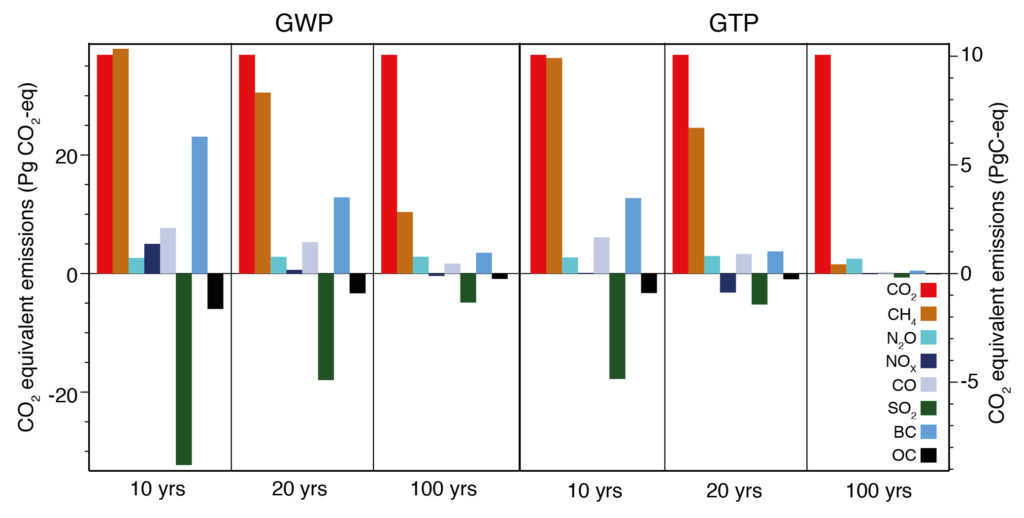
\includegraphics[width=.9\linewidth]{bilder/IPCC_GWP_anthropogenic_emissions.jpg}
			  \caption{Globale von Menschen verursachte Emissionen sortiert nach Klimawirksamkeit (GWP), Quelle: IPCC 2013, Kapitel 8}
		\end{figure}

    \note{
    \begin{itemize}
      \item[] auch Methan bleibt vergleichsweise lange klimawirksam
      \item[] Die wichtigsten anthropogehnen Treibhausgase sind CO$_2$, Methan und Lachgas
      \item[] Sie kommen in sehr unterschiedlichen Konzentration in der Atmospähre vor
      \begin{itemize}
        \item Lachgas bspw. circa 1000 mal weniger als CO$_2$
      \end{itemize}
      \item[] Gleichzeitig ist, bedingt durch ihre molekulare Struktur, ihre Treibhauswirkung ebenfalls sehr unterscheidlich
      \item[] Insgesamt ergibt sich eine vergleichbare Wirkung auf den Treibhauseffekt, ein zusätzliche Strahlungsantrieb (Maß für die Änderung der Energiebilanz der Erde) von etwa \SI{0,2}{\watt\per\square\metre} bis \SI{2}{\watt\per\square\metre}
    	\item[] Darüber hinaus verweilen unterschiedliche Stoffe unterschiedlich lang in der Atmosphäre und sind daher auf unterschiedlichen Zeitskalen wirksam
    	\item[] Auf langen Zeitskalen ist CO$_2$ von hoher Bedeutung
      \item[] GWP = Global Warming Potential
      \item[] GTP = Global Temperature Change Potential
      \item[$\rightarrow$] CO$_2$, CH$_4$ und N$_2$O haben über die Zeit die höchste Klimawirksamkeit
      \item[$\rightarrow$] CO$_2$ verliert über den Zeitraum von 100 Jahren kaum an Klimawirksamkeit
      \item[$\rightarrow$] CO$_2$, CH$_4$ und N$_2$O haben über die Zeit die höchste Klimawirksamkeit
		  \item[$\rightarrow$] CO$_2$ verliert über den Zeitraum von 100 Jahren kaum an Klimawirksamkeit
      \item[] Schwefeldioxid ist ein farbloses, schleimhautreizendes, stechend riechendes und sauer schmeckendes, giftiges Gas
    %		auch Methan bleibt vergleichsweise lange klimawirksam\\
      \end{itemize}
      }

\end{frame}
